\chapter[Implementação do Hardware do Projeto]{Implementação do Hardware do Projeto}

Neste capítulo serão apresentados o desenvolvimento do projeto, seus problemas ocorridos e as tomadas de decisão para implementação do código e do protótipo

\section{Criação de um protótipo para o controle dos poços}

Para teste das ferramentas de controle e automação, serão criados dois tipo de testes: Um teste de sinais e um teste de prototipagem em dimensões pequenas. 
O testes de sinais consiste em testar as saídas e entradas digitais e analógicas em relação ao supervisório, além de testar os registradores ModBus.
Já o tetes em dimensões pequenas será a criação de um protótipo que consiste numa versão diminuta dos problemas levantados pela equipe de engenharia das eclusas.

\section{Especificações do microcontrolador}

O primeiro controlador levantado para a implementação do projeto foi o microcontrolador ATmega328P. Ele é amplamente utilizado em projetos de eletrônica devido às suas características versáteis e robustas, além de sua facilidade de encapsulamento em um sistema embarcado e fácil manutenção por terceiros. Segundo \cite{atmega328p_datasheet} O ATmega328P é baseado na arquitetura AVR de 8 bits e possui as seguintes especificações:

\begin{itemize}
    \item \textbf{Arquitetura}: AVR 8-bit
    \item \textbf{Velocidade de Clock}: até 20 MHz
    \item \textbf{Memória Flash}: 32 KB (com 0,5 KB usados pelo bootloader)
    \item \textbf{SRAM}: 2 KB
    \item \textbf{EEPROM}: 1 KB
    \item \textbf{Pinos de I/O}: 23
    \item \textbf{ADC}: 10-bit, 6 canais (em encapsulamento PDIP) ou 8 canais (em encapsulamento TQFP e QFN/MLF)
    \item \textbf{Interfaces}: USART, SPI, I2C (TWI)
    \item \textbf{Timers}: 2x 8-bit e 1x 16-bit
    \item \textbf{Tensão de Operação}: 1.8V a 5.5V
    \item \textbf{Consumo de Corrente}: 0.2 mA em modo ativo a 1 MHz, 1.8V; 0.1 µA em modo Power-down
    \item \textbf{Temperatura de Operação}: -40°C a 85°C
\end{itemize}

\subsection{Parâmetros de Desempenho Analógico do ATMega28p}

Para a avaliação do desempenho analógico do ATmega328P, são considerados os seguintes parâmetros: Relação Sinal-Ruído (SNR), Relação Sinal-Ruído e Distorção (SINAD), Número Efetivo de Bits (ENOB), Distorção Harmônica Total (THD) e Intervalo Dinâmico Livre de Componentes Espúrias (SFDR).

\subsubsection{Relação Sinal-Ruído (SNR)}

Usando a equação \ref{eq:SNR}, temos para o ADC do ATMEGA 328p:

\[
\text{SNR} = 6.02 \times 10 + 1.76 = 61.96 \, \text{dB}
\]

\subsubsection{Relação Sinal-Ruído e Distorção (SINAD)}

Com a equação \ref{eq:SINAD} achamos  valor exato. Porém, Em um ADC, o SINAD é aproximadamente igual ao SNR.

Então temos:

\[
\text{SINAD} \approx \text{SNR} = 61.96 \, \text{dB}
\]

\subsubsection{Número Efetivo de Bits (ENOB)}

O ENOB pode ser calculado utilizando a euqação \ref{eq:ENOB}. Substituindo o valor de SINAD, temos:

\[
\text{ENOB} = \frac{61.96 - 1.76}{6.02} \approx 9,7 \, \text{bits}
\]


\subsubsection{Distorção Harmônica Total (THD)}

O THD pode ser calculado a partir das distorções harmônicas geradas pelo ADC. A equação \ref{eq:THD} é a referencia para o calculo do THD. Para simplificação, segundo \cite{atmega328p_datasheet} podemos usar um valor típico de THD para o ATmega328P, que é aproximadamente -70 dB.

\subsubsection{Intervalo Dinâmico Livre de Componentes Espúrias (SFDR)}

O SFDR pode ser calculado de acordo com a equação \ref{eq:SFDR}. Para o ATmega328P, segundo \cite{atmega328p_datasheet} o SFDR típico é aproximadamente 61 dB.

\subsection{Resumo dos Valores Calculados}

\begin{itemize}
    \item \textbf{SNR (Relação Sinal-Ruído)}: 61.96 dB
    \item \textbf{SINAD (Relação Sinal-Ruído e Distorção)}: 61.96 dB
    \item \textbf{ENOB (Número Efetivo de Bits)}: 10 bits (ideal), 9,7 bits (prático)
    \item \textbf{THD (Distorção Harmônica Total)}: -70 dB
    \item \textbf{SFDR (Intervalo Dinâmico Livre de Componentes Espúrias)}: 61 dB
\end{itemize}

Esses valores são típicos para um ADC ideal de 10 bits, mas as imperfeições práticas no ATmega328P podem causar variações.

\section{Problemas de desenvolvimento com o ATmega328p}

Com o andar do desenvolvimento do projeto, houveram problemas de desenvolvimento com o ATmega328p e o interfaceamento com a biblioteca <Modbus.h>.

É de suma importância de como um comando Modbus é realizado e como em um controlador ele é enviado. Como discutido no capítulo 02, Um comando Modbus clássico é uma palavra que contém de 8 a 32 bits em data. Os 7 primeiros bytes (ou 56 bits) de uma mensagem transmitida em modbus são a composição PDU como mostrado na figura \ref{fig:teste}. Esse valor é fixo, sendo os dois primeiros Bytes o tipo de transação a ser feita, mais dois bytes de identificação de protocolo mais o tamanho da palavra a ser enviada e um identificador unitário. Como descrito no manual do modbus \cite{modbus2006} a escrita de bobina possui Hexadecimal 0x05, sendo em binário 00000101b. Esse valor é precedido pelo bit de paridade, que pode ser 0 ou 1 e pela escrita em bobina, que também é 0 ou 1. Portanto neste exemplo, um simples comando de identificação de protocolo enviada é 1100000101b, uma palavra simples de 10 bits. Esses valores são o tempo todo modificados e enviados via TCP/IP ou serial RTU.


\begin{figure}[h]
	\centering
	\label{fig:teste}
		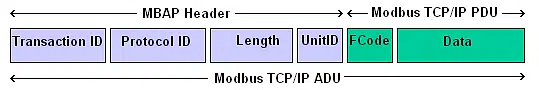
\includegraphics[keepaspectratio=true,scale=0.6]{figuras/tans.jpg}
	\caption{Palavra de comunicação Modbus TCP Fonte:\cite{modbus2006}}
\end{figure}

O compilador do ATMega328P padrão é o AVR-GCC. Este compilador para esta versão de microcontrolador não possui uma implementação de Vector, sendo que a figura \ref{fig:avr_memcpy} um código onde para enviar uma string modbus de forma serializada usando a alocação de memória.

 
\begin{figure}[h]
	\centering
	\label{fig:avr_memcpy}
		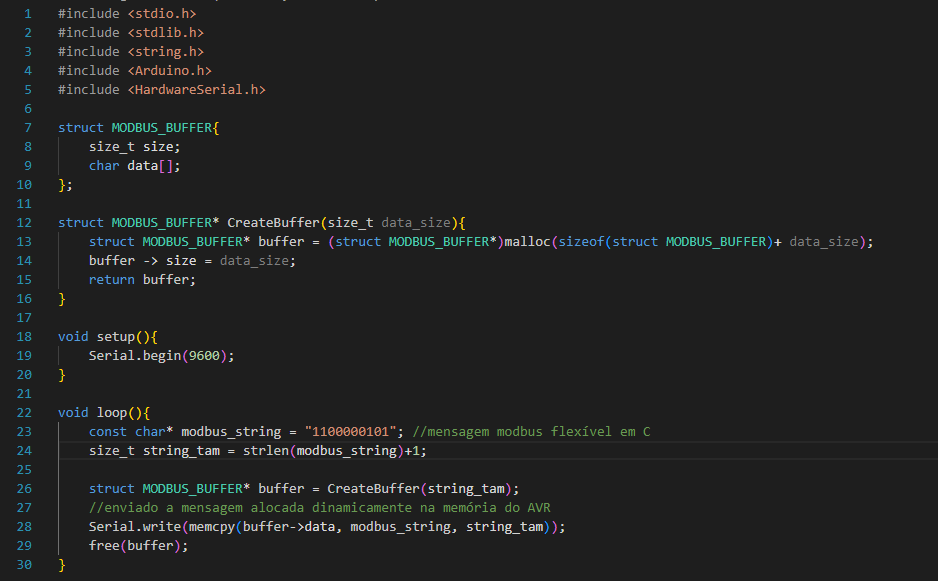
\includegraphics[keepaspectratio=true,scale=0.4]{figuras/memcpy_avr.png}
	\caption{Código com alocação dinâmica de uma string no ATMega328p}
\end{figure}


Como problema com esse tipo de abordagem de código é ter problemas com a memória dinâmica do AVR e com possiveis erros e \textit{overflows}. Uma solução para esse problema é a implementação do método <\textit{Vector}> em que consiste em um array de tamanho dinâmico. A figura \ref{fig:vector} mostra uma implementação em que se usa menos da manipulação da memória física.



\begin{figure}[h]
	\centering
	\label{fig:vector}
		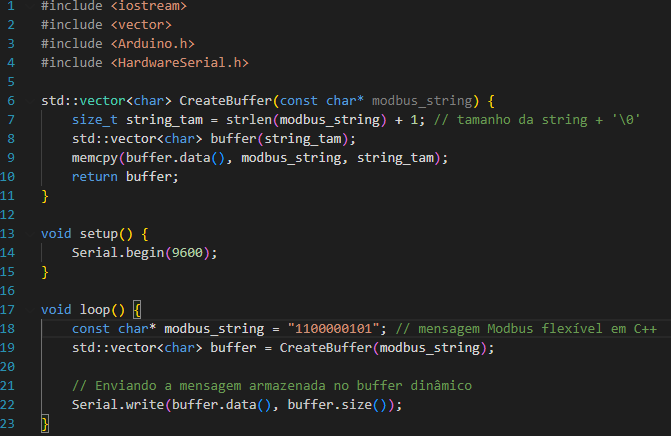
\includegraphics[keepaspectratio=true,scale=0.6]{figuras/vector.png}
	\caption{Código com implementação de Vector em um microcontrolador}
\end{figure}


Com isso, foi escolhido um segundo microcontrolador para a implementação do projeto. O objetivo era um microcontrolador que assim como o ATMega328p pudesse ter fácil manutenção, fácil implementação por parte dos engenheiros com alto código legado. Para essa tarefa foi escolhido o ESP32 com o encapsulamento do tipo WROOM-32, encontrado em kits do tipo NodeMCU. 

\section{O microcontrolador ESP32}

A ESP32 WROOM-32 é um dos módulos mais populares da família ESP32, fabricado pela Espressif Systems. De acordo com \cite{esp32_manual} Ele combina Wi-Fi e Bluetooth, oferecendo uma solução completa para aplicações IoT (Internet of Things). Abaixo estão as especificações principais desse módulo de acordo com o datasheet \cite{esp32_manual}:

\subsection{Dados do processador}
\begin{itemize}
    \item \textbf{Arquitetura:} Xtensa® dual-core 32-bit LX6 microprocessor.
    \item \textbf{Velocidade de Clock:} Até 240 MHz.
    \item \textbf{Memória Flash:} 4 MB (embutido).
    \item \textbf{SRAM:} 520 KB.
    \item \textbf{ROM:} 448 KB.
    \item \textbf{Memória RTC (Real-Time Clock):} 16 KB.
\end{itemize}

Além disso, o ESP32 possui itens adicionais que o ATMega328p não possui, como:

\subsection{Conectividade}
\begin{itemize}
    \item \textbf{Wi-Fi:} 
    \begin{itemize}
        \item 802.11 b/g/n.
        \item Frequência: 2,4 GHz.
        \item Suporte para modo Access Point, Station e modo dual.
    \end{itemize}
    \item \textbf{Bluetooth:}
    \begin{itemize}
        \item Bluetooth v4.2 BR/EDR.
        \item Bluetooth Low Energy (BLE).
    \end{itemize}
\end{itemize}

\subsection{Periféricos}
\begin{itemize}
    \item \textbf{GPIOs:} 34 pinos de GPIO.
    \item \textbf{ADC:} 18 canais de 12 bits.
    \item \textbf{DAC:} 2 canais de 8 bits.
    \item \textbf{Interfaces:} SPI, I2C, I2S, UART, SDIO, PWM.
    \item \textbf{PWM:} 16 canais.
    \item \textbf{Sensores Internos:} Sensor de toque capacitivo, sensor Hall.
\end{itemize}

\subsection{Alimentação}
\begin{itemize}
    \item \textbf{Tensão de Operação:} 3,0V a 3,6V.
    \item \textbf{Consumo de Energia:}
    \begin{itemize}
        \item Modo ativo: $\sim160$ mA @ 240 MHz.
        \item Modo de espera profundo (Deep Sleep): $<10$ µA.
        \item Modo de escuta (Light Sleep): $\sim0.8$ mA.
    \end{itemize}
\end{itemize}

\subsection{Dimensões Físicas}
\begin{itemize}
    \item \textbf{Tamanho:} 18 mm x 25,5 mm x 3 mm.
    \item \textbf{Peso:} Aproximadamente 2,5 g.
\end{itemize}

\subsection{Certificações}
\begin{itemize}
    \item \textbf{Certificações de Regulamentação:} FCC, CE, IC, TELEC, KCC, SRRC, NCC.
\end{itemize}

\subsection{Outras Características}
\begin{itemize}
    \item \textbf{Temperatura de Operação:} -40°C a 85°C.
    \item \textbf{SoC Integrado:} ESP32-D0WDQ6 ou ESP32-D0WD.
    \item \textbf{Suporte para OTA (Over-the-Air) Updates:} Sim.
\end{itemize}

\subsection{Aplicações Típicas}
\begin{itemize}
    \item Dispositivos IoT.
    \item Automação residencial.
    \item Sistemas de monitoramento e controle remoto.
    \item Aplicações com Bluetooth e Wi-Fi integrados.
\end{itemize}

O ESP32 WROOM-32 é conhecido por sua versatilidade e alto desempenho, tornando-o ideal para uma ampla gama de aplicações, especialmente aquelas que exigem conectividade sem fio. Porém, usaremos seu modo RS485 para transmissão de dados para os testes.

\subsection{Parâmetros de Desempenho Analógico}

As especificações de desempenho analógico, como SNR, SINAD, ENOB, THD e SFDR, são importantes para avaliar a qualidade dos conversores analógico-digital (ADC) e digital-analógico (DAC) integrados em microcontroladores como o ESP32 WROOM-32. A seguir, apresento essas especificações com base nas informações disponíveis para o ESP32:

\subsubsection*{Relação Sinal-Ruído (SNR)}
\textbf{Descrição:} O SNR mede a relação entre a potência do sinal útil e a potência do ruído presente no sinal digitalizado.

\textbf{Valor Típico:} Aproximadamente 70 dB para o ADC de 12 bits integrado.

Para um ADC ideal de 12 bits, o SNR pode ser calculado pela fórmula:

\[
\text{SNR}_{\text{ideal}} = 6.02 \times \text{número de bits} + 1.76 \text{ dB}
\]

Para um ADC de 12 bits:

\[
\text{SNR}_{\text{ideal}} = 6.02 \times 12 + 1.76 = 72.24 \text{ dB}
\]

Na prática, o SNR observado pode ser menor devido a ruídos e imperfeições no sistema. Para o ESP32 WROOM-32, um SNR típico observado é em torno de 70 dB.

\subsubsection{Relação Sinal-Ruído e Distorção (SINAD)}
\textbf{Descrição:} O SINAD inclui tanto o ruído quanto a distorção no cálculo, fornecendo uma medida mais abrangente da qualidade do sinal.

\textbf{Valor Típico:} Aproximadamente 67 dB.

O SINAD leva em conta tanto o ruído quanto a distorção harmônica, e é dado por:

\[
\text{SINAD} = 10 \times \log_{10}\left(\frac{P_{\text{signal}}}{P_{\text{noise}} + P_{\text{distortion}}}\right)
\]

Uma relação empírica comum entre SNR e SINAD é:

\[
\text{SINAD} \approx \text{SNR} - 2 \text{ dB}
\]

Portanto, com um SNR de 70 dB, o SINAD pode ser estimado como:

\[
\text{SINAD} \approx 70 - 2 = 68 \text{ dB}
\]

No entanto, devido a imperfeições, um valor típico para o ESP32 é 67 dB.

\subsubsection{Número Efetivo de Bits (ENOB)}
\textbf{Descrição:} O ENOB é uma medida da resolução efetiva do ADC, levando em conta o ruído e a distorção.

\textbf{Valor Típico:} Para o ESP32, o ENOB é geralmente de 10 a 11 bits, dependendo das condições de operação.

O ENOB é uma medida da resolução efetiva de um ADC, levando em conta o SINAD:

\[
\text{ENOB} = \frac{\text{SINAD} - 1.76}{6.02}
\]

Substituindo o valor do SINAD:

\[
\text{ENOB} = \frac{67 - 1.76}{6.02} = \frac{65.24}{6.02} \approx 10.83 \text{ bits}
\]

Arredondando, temos que o ENOB típico do ESP32 é entre 10 e 11 bits.

\subsubsection{Distorção Harmônica Total (THD)}
\textbf{Descrição:} O THD mede a distorção causada por harmônicas indesejadas no sinal digitalizado.

\textbf{Valor Típico:} O THD para o ADC do ESP32 é geralmente inferior a -70 dB, o que indica uma baixa distorção.
Embora o cálculo exato do THD dependa das características específicas do sistema e da forma de onda de entrada, para o ESP32, um valor típico é inferior a -70 dB.

\subsubsection{Intervalo Dinâmico Livre de Componentes Espúrias (SFDR)}
\textbf{Descrição:} O SFDR mede a diferença entre a amplitude do sinal fundamental e a maior espúria não harmônica presente na saída.

\textbf{Valor Típico:} Aproximadamente 70 dB para o ADC do ESP32.

O cálculo exato do SFDR pode envolver medições detalhadas e depende do sinal de entrada e da configuração do ADC, mas para um sistema de 12 bits, o SFDR ideal pode ser próximo do SNR.

\subsection{Resumo dos Valores Típicos para o ESP32 WROOM-32}
\begin{itemize}
    \item \textbf{SNR (Relação Sinal-Ruído):} $\sim$70 dB
    \item \textbf{SINAD (Relação Sinal-Ruído e Distorção):} $\sim$67 dB
    \item \textbf{ENOB (Número Efetivo de Bits):} 10 a 11 bits
    \item \textbf{THD (Distorção Harmônica Total):} $<$ -70 dB
    \item \textbf{SFDR (Intervalo Dinâmico Livre de Componentes Espúrias):} $\sim$70 dB
\end{itemize}

Os valores exatos podem variar dependendo das condições de operação, como a frequência de amostragem, a tensão de alimentação e o ambiente de trabalho. Além disso, as características do PCB (como layout e componentes periféricos) podem impactar o desempenho analógico do ESP32 WROOM-32.

A tabela \ref{tab:comparativo} mostra a diferença entre os controladores ATmega328p e ESP32, o que mostra a superioridade da ESP32 para a aquisição de dados analógicos em relação ao outro controlador.  E a tomada de decisão foi a escolha da ESP32 para prosseguimento do projeto. 

\begin{table}[h!]
\centering
\begin{tabular}{|l|c|c|}
\hline
\textbf{Especificações} & \textbf{ATmega328P} & \textbf{ESP32} \\ \hline
Clock Speed (MHz)       & 20.0                & 240.0          \\ \hline
Flash Memory (KB)       & 32.0                & 4096.0         \\ \hline
SRAM (KB)               & 2.0                 & 520.0          \\ \hline
GPIO Pins               & 23.0                & 34.0           \\ \hline
ADC Channels            & 6.0                 & 18.0           \\ \hline
SNR (dB)                & 55.0                & 70.0           \\ \hline
SINAD (dB)              & 53.0                & 67.0           \\ \hline
ENOB (bits)             & 8.8                 & 10.8           \\ \hline
THD (dB)                & -70.0               & -70.0          \\ \hline
SFDR (dB)               & 55.0                & 70.0           \\ \hline
\end{tabular}
\caption{Comparativo entre ATmega328P e ESP32}
\label{tab:comparativo}
\end{table}


\section{Comandos da bilbioteca modbus.h}
A biblioteca \texttt{Modbus.h} usada no ESP32 é parte da implementação do protocolo Modbus, ela é uma bilbioteca criada por André Sarmento Barbosa e modifcicada por Alexander Emelianov, amplamente utilizado em sistemas industriais e de automação. O endereço da bilioteca é https://github.com/emelianov/modbus-esp8266. Esta biblioteca facilita a comunicação entre dispositivos que suportam o protocolo Modbus, como Controladores Lógicos Programáveis (CLPs), sensores, entre outros dispositivos de automação, sendo até mais fácil de se usar que a biblioteca oficial da Espressif.

\subsection*{Definição de Endereço e Configurações}
\begin{itemize}
    \item \texttt{ModbusRTU modbus;}
    \begin{itemize}
        \item Cria uma instância do Modbus RTU.
    \end{itemize}
    \item \texttt{ModbusTCP modbus;}
    \begin{itemize}
        \item Cria uma instância do Modbus TCP.
    \end{itemize}
\end{itemize}

\subsection{Configurações Gerais}
As configurações gerais servem para inicializar as instâncias do Modbus e para o recebimento dos comandos por um controlador mestre ou por um sistema de supervisório. 
\begin{itemize}
    \item \texttt{modbus.begin(uint8\_t);}
    \begin{itemize}
        \item Inicializa a comunicação Modbus. Para RTU, isso configura a porta serial.
    \end{itemize}
    \item \texttt{modbus.master();}
    \begin{itemize}
        \item Configura o dispositivo como mestre Modbus.
    \end{itemize}
    \item \texttt{modbus.slave(uint8\_t id);}
    \begin{itemize}
        \item Configura o dispositivo como escravo Modbus com o ID especificado.
    \end{itemize}
    \item \texttt{modbus.poll();}
    \begin{itemize}
        \item Deve ser chamado regularmente no loop principal em caso de um sistema de controladores mestre-escravo. Processa as mensagens Modbus e executa ações.
    \end{itemize}
\end{itemize}

\subsection{Funções de Leitura}
As funções de leitura servem basicamente para que um controlador Modbus mestre leia os comandos do controlador escravo. Em um sistema supervisório, esses comandos já são implementados por padrão.
\begin{itemize}
    \item \texttt{modbus.readCoil(uint8\_t id, uint16\_t offset, cbTransaction cb, uint16\_t numregs = 1);}
    \begin{itemize}
        \item Lê o estado de uma ou mais bobinas de um dispositivo escravo.
    \end{itemize}
    \item \texttt{modbus.readDiscrete(uint8\_t id, uint16\_t offset, cbTransaction cb, uint16\_t numregs = 1);}
    \begin{itemize}
        \item Lê o estado de uma ou mais entradas discretas de um dispositivo escravo.
    \end{itemize}
    \item \texttt{modbus.readHoldingRegisters(uint8\_t id, uint16\_t offset, cbTransaction cb, uint16\_t numregs = 1);}
    \begin{itemize}
        \item Lê um ou mais registros de retenção de um dispositivo escravo.
    \end{itemize}
    \item \texttt{modbus.readInputRegisters(uint8\_t id, uint16\_t offset, cbTransaction cb, uint16\_t numregs = 1);}
    \begin{itemize}
        \item Lê um ou mais registros de entrada de um dispositivo escravo.
    \end{itemize}
\end{itemize}

\subsection{Funções de Escrita}
A função de escrita serve para que um controlador mestre escreva um comando para o controlador escravo ou uma escrita de escravo-escravo. Em um software de supervisório, a melhor forma de escrita é por meio de manipulaçao direta de registradores. 
\begin{itemize}
    \item \texttt{modbus.writeCoil(uint8\_t id, uint16\_t offset, bool value, cbTransaction cb);}
    \begin{itemize}
        \item Escreve um valor booleano em uma bobina de um dispositivo escravo.
    \end{itemize}
    \item \texttt{modbus.writeHreg(uint8\_t id, uint16\_t offset, uint16\_t value, cbTransaction cb);}
    \begin{itemize}
        \item Escreve um valor de 16 bits em um registro de retenção de um dispositivo escravo.
    \end{itemize}
    \item \texttt{modbus.writeCoils(uint8\_t id, uint16\_t offset, uint8\_t* value, uint16\_t numregs, cbTransaction cb);}
    \begin{itemize}
        \item Escreve múltiplas bobinas em um dispositivo escravo.
    \end{itemize}
    \item \texttt{modbus.writeHregs(uint8\_t id, uint16\_t offset, uint16\_t* value, uint16\_t numregs, cbTransaction cb);}
    \begin{itemize}
        \item Escreve múltiplos registros de retenção em um dispositivo escravo.
    \end{itemize}
\end{itemize}

\subsection{Funções de Callback}
Uma função de callback serve para que um controlador mestre ou mesmo um supervisório saibam que um comando transicional é realizado (e.g. escrita em um registrador de um mestre para um escravo). O comando de callback é usado para depuração do sistema.
\begin{itemize}
    \item \texttt{void cbTransaction(uint8\_t id, uint8\_t status, uint16\_t* data, uint16\_t len);}
    \begin{itemize}
        \item Função de callback que é chamada quando a transação Modbus é completada. O status da transação pode ser usado para verificar o sucesso ou falha.
    \end{itemize}
\end{itemize}

\subsection{Funções para Configuração de Parâmetros}
São comandos que tem como objetivo de set e preset de transmissão. 
\begin{itemize}
    \item \texttt{modbus.setBaudrate(uint32\_t baudrate);}
    \begin{itemize}
        \item Define a taxa de transmissão para Modbus RTU.
    \end{itemize}
    \item \texttt{modbus.setTimeOut(uint16\_t timeout);}
    \begin{itemize}
        \item Define o tempo limite (timeout) para uma transação Modbus.
    \end{itemize}
    \item \texttt{modbus.setMessageTimeOut(uint16\_t timeout);}
    \begin{itemize}
        \item Define o tempo limite para mensagens.
    \end{itemize}
\end{itemize}

\subsection{Funções para Configuração Avançada}
\begin{itemize}
    \item \texttt{modbus.onDataHandler(cbModbus cb);}
    \begin{itemize}
        \item Define um callback que será chamado ao receber dados Modbus.
    \end{itemize}
    \item \texttt{modbus.onErrorHandler(cbError cb);}
    \begin{itemize}
        \item Define um callback para tratar erros de comunicação.
    \end{itemize}
\end{itemize}

\subsection{Manipulação Direta de Registros Internos}
A manipulação de registradores tem como objetivo a escrita direta de um sistema de supervisório para o controlador escravo. É a forma mais simples e direta de escrita, sendo inclusive de fácil depuração. Para o uso no sistema, será utilizado os métodos de configuração e a manipulação dos registradores de entrada e saída.
\subsubsection{Manipulação de Registros de Retenção (Holding Registers)}
\begin{itemize}
    \item \texttt{mb.Hreg(uint16\_t offset, uint16\_t value = 0);}
    \begin{itemize}
        \item \textbf{Descrição:} Define ou lê o valor de um registro de retenção em uma posição específica (\texttt{offset}).
        \item \textbf{Parâmetros:}
        \begin{itemize}
            \item \texttt{offset}: Posição do registro de retenção.
            \item \texttt{value}: (Opcional) Valor a ser definido no registro. Se não for fornecido, a função retorna o valor atual do registro.
        \end{itemize}
        \item \textbf{Exemplo:}
        \begin{verbatim}
mb.Hreg(100, 12345); // Define o valor 12345 no registro de retenção 100
uint16_t value = mb.Hreg(100); // Lê o valor do registro de retenção 100
        \end{verbatim}
    \end{itemize}
\end{itemize}

\subsubsection{Manipulação de Entradas Discretas (Discrete Inputs)}
\begin{itemize}
    \item \texttt{mb.Ists(uint16\_t offset, bool value = 0);}
    \begin{itemize}
        \item \textbf{Descrição:} Define ou lê o estado de uma entrada discreta em uma posição específica (\texttt{offset}).
        \item \textbf{Parâmetros:}
        \begin{itemize}
            \item \texttt{offset}: Posição da entrada discreta.
            \item \texttt{value}: (Opcional) Estado a ser definido na entrada. Se não for fornecido, a função retorna o estado atual da entrada.
        \end{itemize}
        \item \textbf{Exemplo:}
        \begin{verbatim}
mb.Ists(10, true); // Define o estado da entrada discreta 10 para true (ligado)
bool state = mb.Ists(10); // Lê o estado da entrada discreta 10
        \end{verbatim}
    \end{itemize}
\end{itemize}

\subsubsection{Manipulação de Bobinas (Coils)}
\begin{itemize}
    \item \texttt{mb.Coil(uint16\_t offset, bool value = 0);}
    \begin{itemize}
        \item \textbf{Descrição:} Define ou lê o estado de uma bobina em uma posição específica (\texttt{offset}).
        \item \textbf{Parâmetros:}
        \begin{itemize}
            \item \texttt{offset}: Posição da bobina.
            \item \texttt{value}: (Opcional) Estado a ser definido na bobina. Se não for fornecido, a função retorna o estado atual da bobina.
        \end{itemize}
        \item \textbf{Exemplo:}
        \begin{verbatim}
    mb.Coil(5, true); // Define o estado da bobina 5 para true (ligado)
    bool coilState = mb.Coil(5); // Lê o estado da bobina 5
        \end{verbatim}
    \end{itemize}
\end{itemize}

\subsubsection{Manipulação de Registros de Entrada (Input Registers)}
\begin{itemize}
    \item \texttt{mb.Ireg(uint16\_t offset, uint16\_t value = 0);}
    \begin{itemize}
        \item \textbf{Descrição:} Define ou lê o valor de um registro de entrada em uma posição específica (\texttt{offset}).
        \item \textbf{Parâmetros:}
        \begin{itemize}
            \item \texttt{offset}: Posição do registro de entrada.
            \item \texttt{value}: (Opcional) Valor a ser definido no registro. Se não for fornecido, a função retorna o valor atual do registro.
        \end{itemize}
        \item \textbf{Exemplo:}
        \begin{verbatim}
mb.Ireg(50, 6789); // Define o valor 6789 no registro de entrada 50
uint16_t inputValue = mb.Ireg(50); // Lê o valor do registro de entrada 50
        \end{verbatim}
    \end{itemize}
\end{itemize}


\section{Implementação do código e testes de sinais}

Para implementação do código, serão separados em 3 partes: A lógica de como os motores dos poços funcionarão, a lógica dos semáforos da jusante e montante e a lógica da ponte. O código do projeto irá usar a biblioteca \texttt{<Arduino.h>} e toda a lógica consagrada pela fundação Arduino. O objetivo de uso é a facilidade de código legado, para que um operador, ou mesmo um outro engenheiro possa trabalhar no sistema. 

A lógica dos motores consiste no sistema possuir 3 motores em que são acionados com a subida do nível do sistema, conforma demonstrado na figura \ref{fig:diag_pocos}. Partindo do pressuposto da existência de sensores analógicos, o controle do sinal analógico será dado pelo registrador de retenção \texttt{mb.Hreg()}. É através dele que serão lidos os valores analógicos do sistema. Para os motores, podemos utliziar tanto registradores de entrada discreta como registradores de bobina. Como uma decisão de projeto, e por se tratar de um acionamento, será utilizado no código o acionamento de bobinas \texttt{mb.Coil()}. Para o acionamento dos semáforos da jusante e da montante, será também utilizado registradores de manipulação de boninas. Para a ponte, que consiste em um motor de passo com um conjunto de fim de curso, que seu acionamento se dará pelo registrador de coil e para os fim de curso será utilizado a manipulação de entrada discreta \texttt{mb.Ists()}.

Com isso, será usado o controlador como modo \textit{slave} (slave ID 1) e serão separados os registradores da seguinte forma:

\begin{itemize}
    \item Registradores dos motores dos poços e sensor: 101, 102, 103 e 104
    \item Registradores dos semáforos: 201, 202, 203, 204, 205 e 206
    \item Registradores dos itens da ponte: 301, 302, 303 e 304
\end{itemize}

A separação dessa forma serve para melhor depurar o projeto por parte dos controladores e operadores das eclusas. Será usado a diretiva de compilação \texttt{define} como boa prática de programação. Então, será feito \texttt{define MOTOR\_01 101} como diretiva para que o valor do registrador seja salvo na variável diretiva. Com isso, os métodos \texttt{mb.addCoil()}, \texttt{mb.addHreg()}, \texttt{mb.addIreg()} serão adicionados no \texttt{void setup()} do código. 

\begin{figure}[h]
	\centering
	\label{fig:esp_32_pinout}
		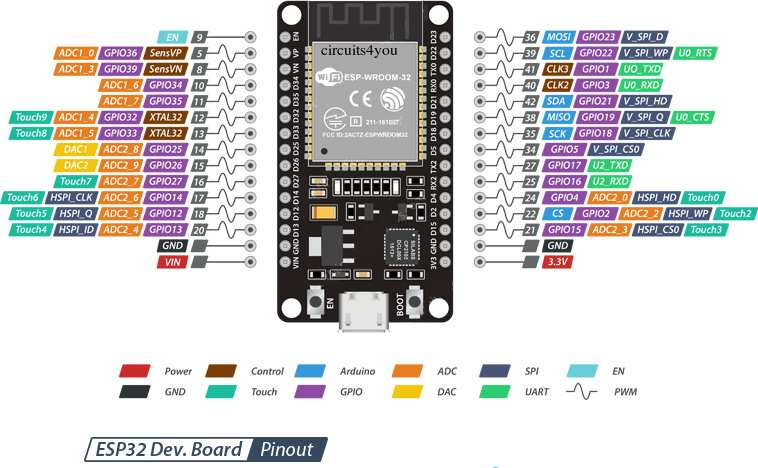
\includegraphics[keepaspectratio=true,scale=0.6]{figuras/ESP32-Pinout.jpg}
	\caption{Pinagem do esp32 (fonte: https://circuits4you.com/)}
\end{figure}

A figura \ref{fig:esp_32_pinout} mostra as GPIOs disponíveis para o controlador, suas funções analógicas e digitais, assim como as portas de comunicação I²C e UART (Serial). Para igualar os registradores com os pinos da ESP32, utilizaremos os pinos 39,34, 35 e 36 para os registradores 101 a 104; pinos 16, 17, 18, 19, 21 e 5 para os registradores 201 a 206 e pinos 33, 25, 26 e 9 para os registradores 301 a 304.

Para cada ação, será usado no \textit{loop} principal quatro funções. A primeira será \texttt{lerSensor()}, que tem por objetivo ler o sensor analógico pelo método \texttt{analogRead()}, com a leitura do pino do sensor e a escrita no registrador (\texttt{analogRead(SENSOR\_PIN, mb.Hreg(SENSOR))}. A segunda e a terceira função \texttt{acionarMotor()} e \texttt{acionarSemaforos()} possuem o mesmo objetivo, que é a escrita nas coils dos valores dos motores e dos semáforos. Utilizando o método \texttt{digitalWrite(pino, Registador)} será a forma de escrita via controlador.

Para o método \texttt{acionarPonte()}, será adicionado um botão do tipo digital no supervisório. este botão será lido pelo controlador pelo registrador 302 e a partir do acionamento será movido o motor. Para a movimentação do motor de passo, será usado a biblioteca \texttt{<AccelStepper.h>}. Os valores do motor serão configurados pelo construtor \texttt{AccelStepper motor(AccelStepper::DRIVER, MOTOR\_PASSO\_EN\_PIN, MOTOR\_PASSO\_DIR\_PIN)} e no \textit{setup} serão configurados a velocidade do motor e sua aceleração. A função então testará se o botão digital será acionado, e se acionado, verificar os fins de curso e assim mover o motor. 

O Anexo A possui o código completo para ser implementado e compilado. 


\section{Implementação o protótipo }

Para implementação do projeto para simulação de sinais e para a criação de um protótipo de apresentação, o projeto será prototipado em uma placa do tipo \textit{protoboard}. Os motores para a simulação das bombas serão três bombas DC de operação de 5V DC. Para os semáforos, serão utilizados um conjunto de 6 \textit{LEDs} de cores Vermelho, Amarelo e Verde e para o motor da ponte será usado um servo motor DC. O teste de paradigma tem como objetivo a demonstração de resultados que podem ser usados em um modelo de maior escala usando o mesmo código com poucas modificações.

\subsection{Acionamento das bombas DC}

Para o acionamento das bombas DC, será realizado o \textit{drive} do motor DC. De acordo com \cite{hashid} Um \textit{drive} de motor DC é um dispositivo eletrônico usado para controlar a velocidade, direção e torque de motores de corrente contínua (DC). O \textit{drive} regula a quantidade de corrente e a tensão fornecida ao motor, ajustando a potência de acordo com a necessidade de aplicação.

Para a aplicação do sistema, o acionamento será direto (Ou seja, sem o uso de PWM). O \textit{drive} servirá para a proteção do circuito e para o melhor acionamento dos motores. Para isso, um transistor do tipo MOSFET será usado como uma chave eletrônica para o acionamento dos motores DC. Para maior segurança, um diodo será colocado entre os polos do motor para aumentar a segurança contra corrente reversa e um divisor de tensão será colocado para que a tensão seja sempre 3.3 volts no \textit{Gate}.

\subsubsection{Escolha de um transistor para o acionamento}

A escolha do transistor a principio foi uma escolha de um componente comumente usado para realizar o \textit{drive} de motores. A primeira escolha foi do MOSFET IRF1404, porém, de acordo com o datasheet do IRF1404 \cite{IRF1404_datasheet} a tensão $V_{GS}$ de \textit{threshold} é em torno de 2 a 4 Volts. Para um bom acionamento, ou seja, para funcionamento em modo de saturação, a tensão $V_{GS}$ tem que ser maior que a tensão tensão $V_{GS}$ de \textit{threshold}, e o IRF1404 tipicamente possui uma tensão de 10V para que a resistencia $R_{DS(on)}$ seja mínima.

Com isso, foi realizado uma pesquisa de componentes no mercado para o acionamento e o mais adequado é utilizar um transistor do tipo \textit{Logic-Level}, onde seu acionamento se dá por níveis lógicos de 3,3V ou 5V e seu $V_{GS}$ de \textit{threshold} seja menor que $V_{GS}$. Então como resultado foi usado o MOSFET IRLZ44N, que seu $V_{GS(Th)}$ é entre 1 e 2V.


\subsection{Esquemático dos itens do projeto}

\begin{figure}[h]
	\centering
	\label{fig:motor_esquema}
		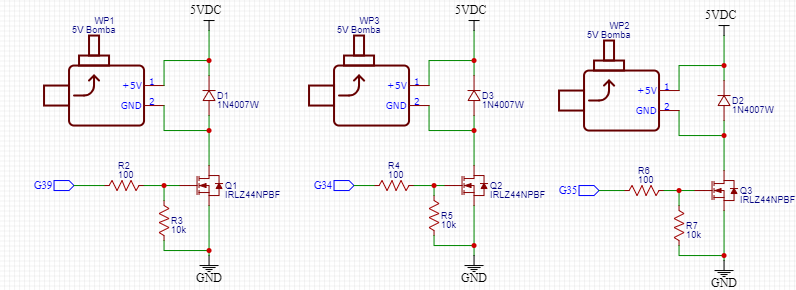
\includegraphics[keepaspectratio=true,scale=0.6]{figuras/motores.png}
	\caption{Esquemático das bombas DC}
\end{figure}

\begin{figure}[h]
	\centering
	\label{fig:LEDs_esquema}
		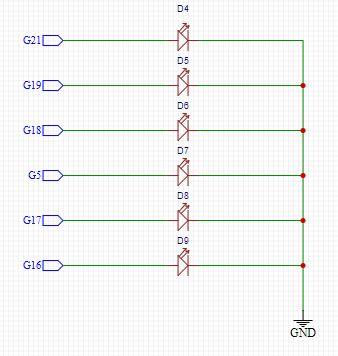
\includegraphics[keepaspectratio=true,scale=0.8]{figuras/leds.png}
	\caption{Esquemático dos LEDs}
\end{figure}

\begin{figure}[h]
	\centering
	\label{fig:Servo_esquema}
		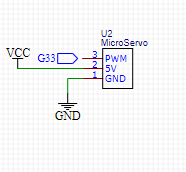
\includegraphics[keepaspectratio=true,scale=0.8]{figuras/servo.png}
	\caption{Esquemático do Servo Motor}
\end{figure}

A figura \ref{fig:motor_esquema} mostra como ficou o resultado da montagem de cada uma das bombas DC no sistema. Para o aumento de proteção, foi usado um diodo 1N4007 para evitar corrente reversa e um divisor de tensão na entrada para que o valor seja fixo em 3,3V e dar mais uma camada de proteção ao sistema. Para a simulação de um sensor analógico, foi colocado um potênciometro de 10k$\Omega$ conectado a GPIO G32 que fará o trabalho da variação do sinal analógico no conversor AD.
Para a colocação dos LEDs, foram usados três leds do tipo Vermelho, Amarelo e Verde. Não foram colocados resistores. O servo motor foi colocado na porta G35 e seu acionamento para este caso será por PWM.




